\documentclass{../source/Experiment}

\major{信息工程}
\name{姚桂涛}
\title{常用组合电路模块的设计和应用}
\stuid{3190105597}
\college{信息与电子工程学院}
\date{\today}
\lab{东4-223}
\course{数字系统实验设计}
\instructor{屈民军、唐奕}
\grades{}
\expname{}
\exptype{}
\partner{}
\begin{document}
    \makecover

    \section{实验目的}
        \begin{enumerate}
            \item 掌握音符产生的方法,了解 DDS技术的应用。
            \item 了解音频编解码的应用。
            \item 掌握系统“自顶而下”的数字系统设计方法。
        \end{enumerate}
    \section{实验任务}
        设计一个音乐播放器,要求以下条件。
        \begin{enumerate}
            \item 可以播放四首乐曲,设置play/pause \_ button、next \_ button、reset 三个按键。按play/pause \_ button键,音乐在播放和暂停之间切换;按next \_ button 键播放下一首乐曲。
            \item LEDO指示播放情况(播放时点亮)、LED2和LED 3指示当前乐曲序号。
        \end{enumerate}
    \section{实验原理}

        根据实验任务可将系统划分为时钟管理模块(DCM)、按键处理、主控制器、乐曲读取、音符播放(note \_ player)、同步化电路、节拍基准产生器和音频编解码接口电路等子模块。
        
        时钟管理模块(DCM)产生100MHz的系统时钟sys \_ clk和 12.5MHz的音频时钟audio \_ clk。
        
        主控制器(mcu)模块接收按键信息,通知 song \_ reader模块是否要播放(play)及播放哪首乐曲(song)。
        
        乐曲读取(song \_ reader)模块根据mcu模块的要求,逐个取出音符信息{note,duration}送给note \_ player模块播放,当一首乐曲播放完毕,回复mcu模块乐曲播放结束信号(song \_ done)。

        音符播放接收到需播放的音符,在音符的持续时间内,以48kHz速率送出该音符的正弦波样品给音频编解码接口模块。当一个音符播放结束,向 song \_ reader模块发送一个note \_ done脉冲索取新的音符。

        音频编解码接口模块负责将音符的正弦波样品转换为串行输出并发送给音频编解码芯片 \\ ADAU1761。音频编解码芯片ADAU1761接收正弦波样品,再进行AD转换并放大,最后送至扬声器播放。注意,note \_ player模块产生的正弦波样品为16位二进制,需在低位加8个0后送入音频编解码接口模块。

        由于音频编解码模块与系统使用不同时钟,因此需要同步化电路协调两部分电路。
            
        节拍基准产生器产生48Hz的节拍定时基准脉冲信号(beat),而 ready信号频率为48kHz,因此,节拍基准产生器为分频比为1000的分频器。而按键处理模块完成输入同步化、防颤动和脉宽变换等功能。

        \subsection{具体设计}
            \subsubsection{主控制模块mcu的设计}

                主控制模块mcu有响应按键信息、控制系统播放两大任务,表6.11为其端口含义。

                \begin{table}[H]
                    \caption{主控制模块mcu的端口含义}
                    \begin{tabular}{|c|c|p{0.73\textwidth}|}
                        \hline
                        引脚名称          & I/O    & \multicolumn{1}{c|}{引脚说明}                                    \\ \hline
                        clk           & Input  & 100MHz时钟信号                                                   \\ \hline
                        reset         & Input  & 复位信号,高电平有效                                                   \\ \hline
                        play\_pause   & Input  & 来自按键处理模块的“播放/暂停”控制信号,一个时钟周期宽度的脉冲                             \\ \hline
                        next          & Input  & 来自按键处理模块的“下一曲”控制信号,一个时钟周期宽度的脉冲                               \\ \hline
                        play          & Output & 输出控制信号,高电平表示播放,控制song \_reader模块是否要播放                        \\ \hline
                        reset\_play   & Output & 时钟周期宽度的高电平复位脉冲reset play,用于同时复位模块song\_reader和 note\_ player \\ \hline
                        song\_done    & Input  & song\_ reader模块的应答信号,一个时钟周期宽度的高电平脉冲,表示一曲播放结束                 \\ \hline
                        song{[}1:0{]} & Output & 当前播放乐曲的序号                                                    \\ \hline
                    \end{tabular}
                \end{table}
                根据设计要求,模块mcu的原理框图如图所示。图中的2位二进制数用来计算乐曲序号(song)。

                \begin{figure}[H]
                    \centering
                    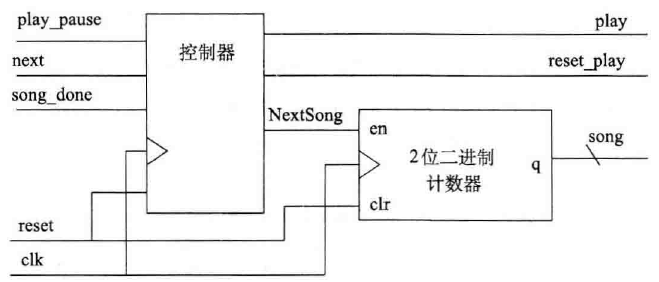
\includegraphics[width = 0.8\textwidth]{pic/mcu.png}
                    \caption{mcu的结构框图}
                \end{figure}

                根据原理框图设计出mcu顶层代码如下:
                \lstinputlisting[
                    language  =   Verilog,
                    title     =   {mcu顶层代码}
                ]{src/mcu.v}

                控制器的工作流程图如图6.46所示,控制器设置初始复位(RESET)、播放(PLAY)、暂停(PAUSE)和下一首(NEXT)四种状态。系统复位后,经RESET状态初始化后进入PAUSE状态,等待各种命令输入; play \_ pause脉冲信号使系统在 PLAY、PAUSE两状态之间互转;在 PLAY或 PAUSE 状态下,若按下next \_ button按钮,则使系统在进入NEXT状态,输出reset \_  play脉冲复位song  \_ reader和 note \_ player两个模块,同时输出脉冲 NextSong 乐曲序号计数器加1,进入下一曲播放;另外,在PLAY状态时,若乐曲播放结束(song \_ done有效)则结束播放,经 RESET状态复位 song \_ reader和 note \_ player两个模块,并进入 PAUSE状态,再次等待各种命令输入。

                \begin{figure}[H]
                    \centering
                    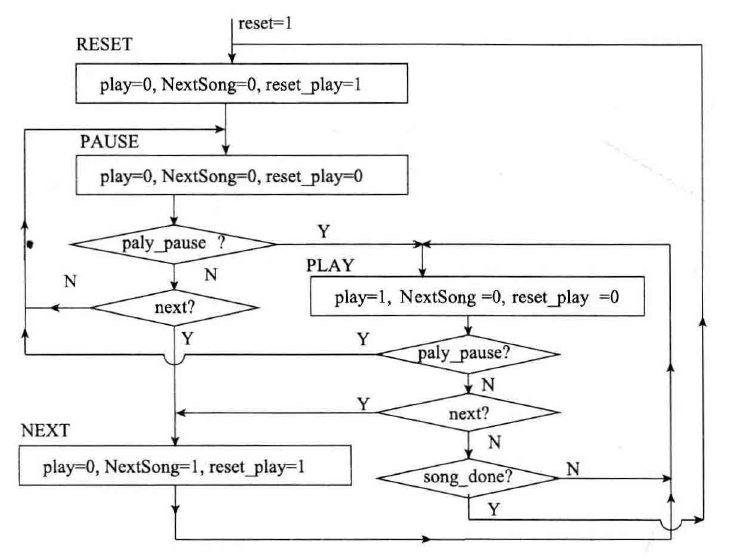
\includegraphics[width = 0.8\textwidth]{mcu-c}
                    \caption{mcu控制器的算法流程}
                \end{figure}

                根据原理框图设计出mcu控制器代码如下:
                \lstinputlisting[
                    language  =   Verilog,
                    title     =   {mcu控制器代码}
                ]{src/mcu_controller.v}

            \subsubsection{乐曲读取模块song \_ reader的设计}

                乐曲读取模块song \_ reader的任务有
                (1)根据mcu模块的要求,选择播放乐曲。
                (2)响应note \_ player模块请求,从 song \_ rom中逐个取出音符{note,duration}送给note \_ player模块播放。
                (3)判断乐曲是否播放完毕,若播放完毕,则回复mcu模块应答信号。根据 song \_ reader模块的任务要求,song \_ reader模块需包含表6.12所示的输入、输出端口。

                \begin{table}[H]
                    \caption{乐曲读取模块song \_ reader的端口含义}
                    \begin{tabular}{|c|c|p{0.72\textwidth}|}
                        \hline
                        引脚名称              & I/O    & \multicolumn{1}{c|}{引脚说明}                        \\ \hline
                        clk               & Input  & 100MHz时钟信号                                       \\ \hline
                        reset             & Input  & 复位信号,高电平有效                                       \\ \hline
                        play              & Input  & 来自mcu的控制信号,高电平要求播放                               \\ \hline
                        song{[}1:0{]}     & Input  & 来自mcu的控制信号,当前播放乐曲的序号                             \\ \hline
                        note\_done        & Input  & 即模块note player的应答信号,一个时钟周期宽度的脉冲,表示一个音符播放结束并索取新音符 \\ \hline
                        song\_done        & Output & 给mcu 的应答信号,当乐曲播放结束,输出-一个时钟周期宽度的脉冲,表示乐曲播放结束       \\ \hline
                        note{[}5:0{]}     & Output & 音符标记                                             \\ \hline
                        duration{[}5:0{]} & Output & 音符的持续时间                                          \\ \hline
                        new\_note         & Output & 给模块note\_playe的控制信号,一个时钟周期宽度的高电平脉冲,表示新的音符需播放     \\ \hline
                    \end{tabular}
                \end{table}

                song \_ rom是一个只读存储器,用来存放乐曲,容量为2'×12bits。共存放四首乐曲,每首乐曲占用25×12bits空间,即每首乐曲最长由32个音符组成。因此,song \_ rom高2位地址决定哪首乐曲,而低5位地址决定这首乐曲的哪个音符。song \_ rom每个地址存放一个音符信息,音符信息由12位二进制组成,高6位表示音符标记note,低 6位表示音长duration。 
                
                song \_ rom模块已由作者提供,前三首乐曲已填写,第4首乐曲空白,由读者自己填写,这里说明一下,若乐曲不足 32个音符,多余的空间用数字0填补。
                
                根据song \_ reader模块的功能及song  \_ rom结构,可画出图6.47所示的结构框图,控制器主要负责接收mcu模块与note \_ player模块的控制信号,并做出响应。算法流程图如图6.48所示。

                \begin{figure}[H]
                    \centering
                    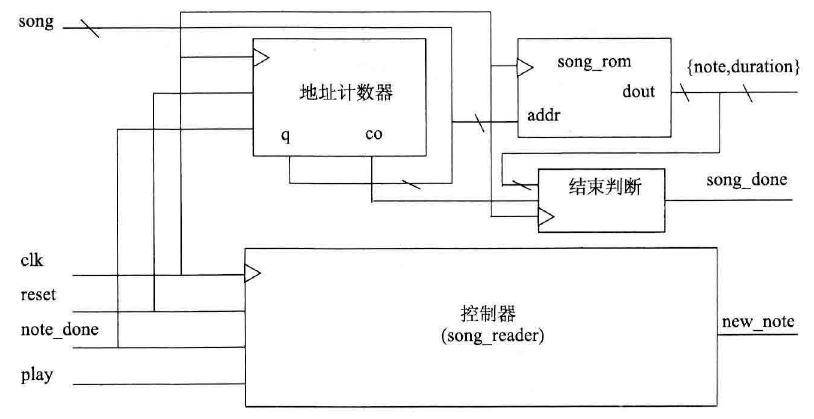
\includegraphics[width = 0.8\textwidth]{song}
                    \caption{song \_ reader的结构框图}
                \end{figure}

                根据原理框图设计出song \_ reader顶层代码如下:
                \lstinputlisting[
                    language  =   Verilog,
                    title     =   {song \_ reader顶层代码}
                ]{src/song_reader.v}

                系统复位后一直在RESET状态等待mcu模块控制信号输入,当mcu模块发出播放命令(play为高电平)时,进入NEW \_ NOTE状态输出new \_ note脉冲要求note \_ player模块播放音符;然后进入 WAIT状态等待,当note \_ player模块播放完音符时,会发出note \_ done脉冲信号索取下一音符,note \_ done脉冲信号一方面让地址计数器递增,并从 song \_ rom 取出一个新的音符,另一方面让控制器进入NEW \_ NOTE状态,输出new \_ note脉冲通知 note \_ player模块有新的音符需要播放。当note \_ done有效,需要两个时钟周期才能从song \_ rom中读取下一个音符信息。因此新音符有效标记信号new \_ note也应在新音符数据输出后有效,其时序关系如图6.49所示。所以在流程图中插入NEXT \_ NOTE状态,目的是延迟一个时钟周期输出信号,以配合song \_ rom的读取要求。

                地址计数器为5位二进制计数器,其中 note \_ done为计数使能输入,当note \_ done为高电平时,允许计数。计数器状态q为song \_ rom 的低5位地址,song[ 1:0]为song  \_ rom高两位地址。
                
                当地址计数器出现进位或duration为0时,表示乐曲结束,应输出一个时钟周期宽度的高电平脉冲信号song \_ done。

                \begin{figure}[H]
                    \centering
                    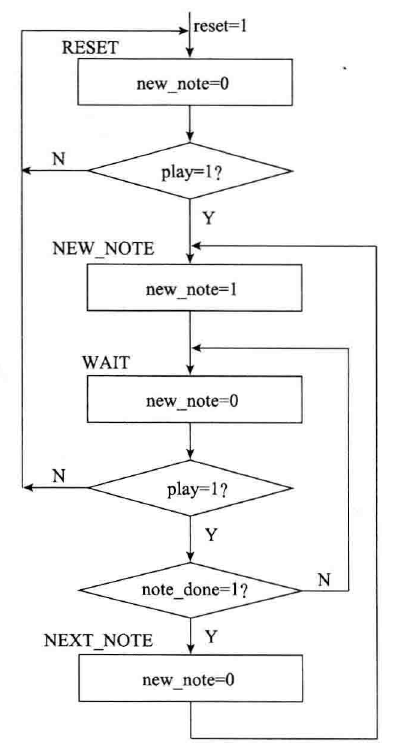
\includegraphics[width = 0.3\textwidth]{song-c}
                    \caption{song \_ reader控制器的算法流程}
                \end{figure}

                根据原理框图设计出song \_ reader控制器代码如下:
                \lstinputlisting[
                    language  =   Verilog,
                    title     =   {song \_ reader控制器代码}
                ]{src/song_reader_controller.v}
               
            \subsubsection{音符播放模块note \_ player的设计}

                音符播放模块note \_ player是本实验的核心模块,它主要任务包括以下几方面。
                (1)从song \_ reader模块接收需播放的音符{note, duration}。
                (2)根据note值找出 DDS的相位增量k。
                (3)以48kHz速率从Sine ROM取出正弦样品送给音频编解码器接口模块。
                (4)当一个音符播放完毕,向song \_ reader模块索取新的音符。
                
                根据note \_ player模块的任务,进一步划分功能单元,如图6.50所示,图中FreqROM为只读存储器,完成音符标记 note 与 DDS模块的相位增量k查找表关系。表6.13所示为note \_ player模块的端口含义。

                \begin{figure}[H]
                    \centering
                    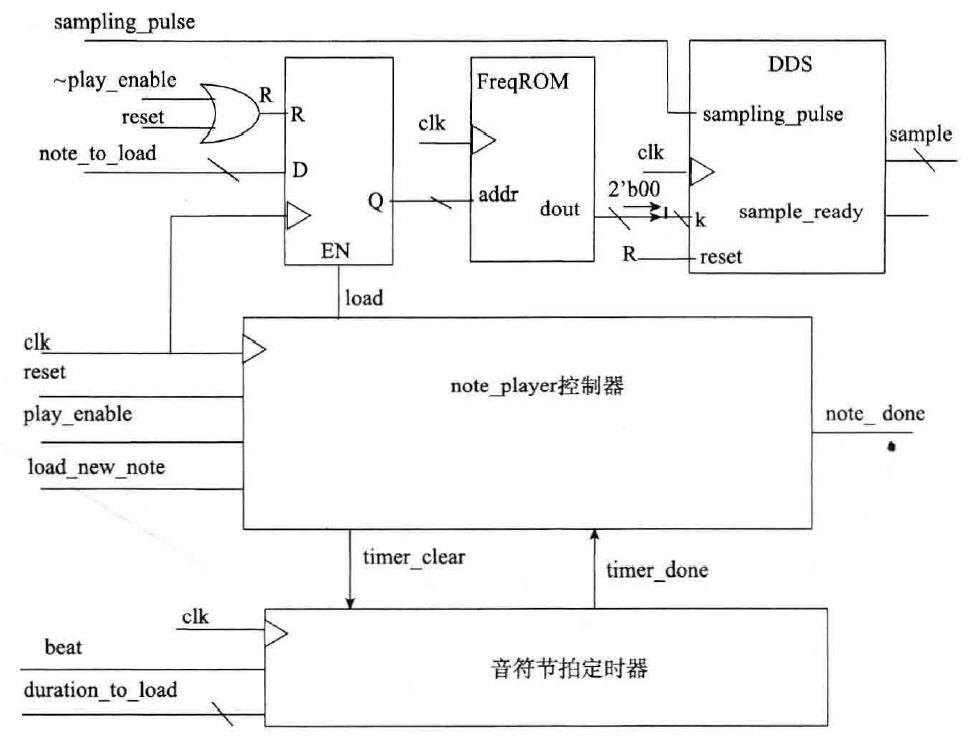
\includegraphics[width = 0.8\textwidth]{note}
                    \caption{note \_ player的结构框图}
                \end{figure}

                \begin{table}[H]
                    \caption{note \_ player 模块的端口含义}
                    \begin{tabular}{|c|c|p{0.62\textwidth}|}
                        \hline
                        引脚名称                        & I/O    & \multicolumn{1}{c|}{引脚说明}                              \\ \hline
                        clk                         & Input  & 系统时钟信号,外接sys\_clk                                      \\ \hline
                        reset                       & Input  & 复位信号,高电平有效,外接mcu模块的reset\_ play                        \\ \hline
                        play\_enable                & Input  & 来自mcu模块的play信号,高电平表示播放                                 \\ \hline
                        note\_to\_load{[}5:0{]}     & Input  & 来自song\_reader模块的音符标记note,表示需播放的音符                     \\ \hline
                        duration\_to\_load{[}5:0{]} & Input  & 来自 song \_reader模块的音符持续时间duration,表示需播放音符的音长           \\ \hline
                        load\_new\_note             & Input  & 来自 song\_reader模块的new\_note信号,一个时钟周期宽度的高电平脉冲,表示新的音符需播放 \\ \hline
                        note\_done                  & Output & 给song\_reader模块的应答信号,一个时钟周期宽度的高电平脉冲,表示音符播放完毕           \\ \hline
                        sampling\_pulse             & Input  & 来自同步化电路模块的ready信号,频率48kHz,一个时钟周期宽度的高电平脉冲,表示索取新的正弦样品    \\ \hline
                        beat                        & Input  & 定时基准信号,频率为48Hz脉冲,一个时钟周期宽度的高电平脉冲                        \\ \hline
                        sample{[}15:0{]}            & Output & 正弦样品输出                                                 \\ \hline
                    \end{tabular}
                \end{table}

                根据原理框图设计出note \_ player顶层代码如下:
                \lstinputlisting[
                    language  =   Verilog,
                    title     =   {note \_ player顶层代码}
                ]{src/note_player.v}
               
                

                note \_ player控制器负责与song \_ reader模块接口,读取音符信息,并根据音符信息从Frequency ROM中读取相应相位增量k送给DDS子模块。另外,note \_ player控制器还需要控制音符播放时间。note \_ player控制器的算法流程如图6.51所示。在复位或未播放时,控制器处于RESET状态或PLAY状态,由于此时高电平reset或低电平play \_ enable都使图6.35中的D型寄存器清0,进而使k为0,不会输出正弦样品。当play \_ enable为高电平,系统进入音符播放PLAY状态,当一个音符播放结束时,控制器进入DONE状态,置位done \_ with \_ note,向 song \_ reader模块索取新的音符,此时song \_ reader模块输出一个new \_ note脉冲信号使控制器进入LOAD状态,读取新的音符,然后进入 PLAY状态播放下一个音符。

                音符定时器为6位二进制计数器,beat、timer \_ clear分别为使能、清О信号,均为高电平有效。定时时间由音长信号 duration \_ to \_ load决定,即duration \_ to \_ load个beat周期, timer \_ done为定时结束标志。
                子模块 DDS的功能就是利用DDS技术产生正弦样品,其工作原理已在实验15中介绍了,注意:DDS模块的输入k为22位二进制,因此需FreqROM输出的20位相位增量高位加2个0后接入DDS。

                \begin{figure}[H]
                    \centering
                    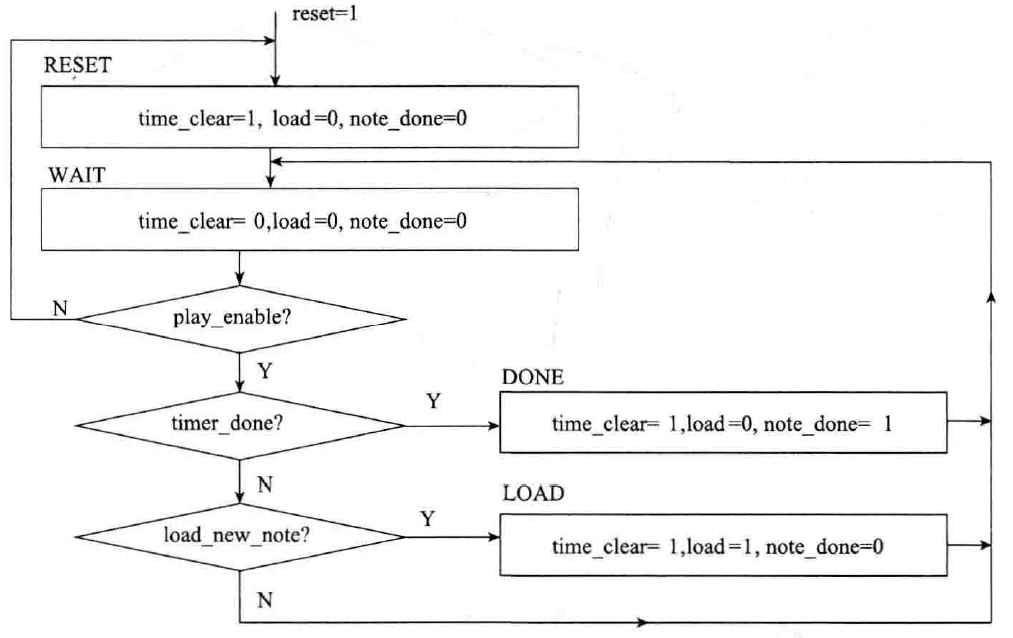
\includegraphics[width = 0.8\textwidth]{note-c}
                    \caption{note \_ player控制器的算法流程}
                \end{figure}
                
                根据原理框图设计出note \_ player控制器代码如下:
                \lstinputlisting[
                    language  =   Verilog,
                    title     =   {note \_ player控制器代码}
                ]{src/note_player_controller.v}
            \subsubsection{同步化电路}

                由于音频编解码接口模块和其他模块采用不同的时钟,因此两者之间的控制及应答信号须进行同步化处理。
                本例中音频编解码接口模块的输出信号NewFrame的脉冲宽度为一个audio \_ clk 时钟周期,需通过同步化处理,产生与sys \_ clk同步且脉冲宽度为一个sys \_ clk时钟周期的信号ready。电路如图6.52所示,由同步器和脉冲宽度变换电路组成。

                \begin{figure}[H]
                    \centering
                    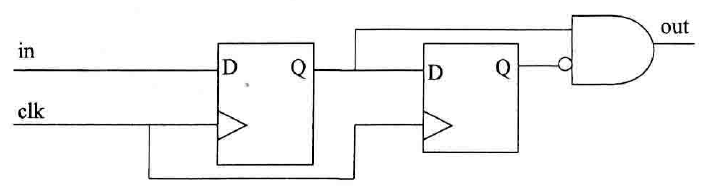
\includegraphics[width = 0.6\textwidth]{syc}
                    \caption{同步化电路}
                \end{figure}

                同步化电路代码如下:
                \lstinputlisting[
                    language  =   Verilog,
                    title     =   {同步化电路代码}
                ]{src/synchro.v}
            
            \subsubsection{时钟管理模块(DCM)}
        
                IP内核时钟管理模块的输入时钟 clk频率为100MHz,产生100MHz的系统时钟和12.50MHz的音频时钟。
                
                另外,音频编解码接口模块与按键处理模块按实验18和实验11介绍设计。也可调用作者提供的设计。不过,作者是以 BlackBox方式提供,即音频编解码接口模块提供综合网表文件AudioInterface.edf 和端口文件AudioInterface.v;而按键处理模块提供综合网表文件button press \_ unit.edf和端口文件button \_ press \_ unit.v。

    \section{主要仪器设备}
    Modelsim SE、Vivado、Nexys Video Artix-7 FPGA多媒体音视频智能互联开发系统、有源音响或耳机。
    \section{实验过程}
        \subsection{仿真测试}
            \subsubsection{主控制器mcu模块}
            仿真图:
                \begin{figure}[H]
                    \centering
                    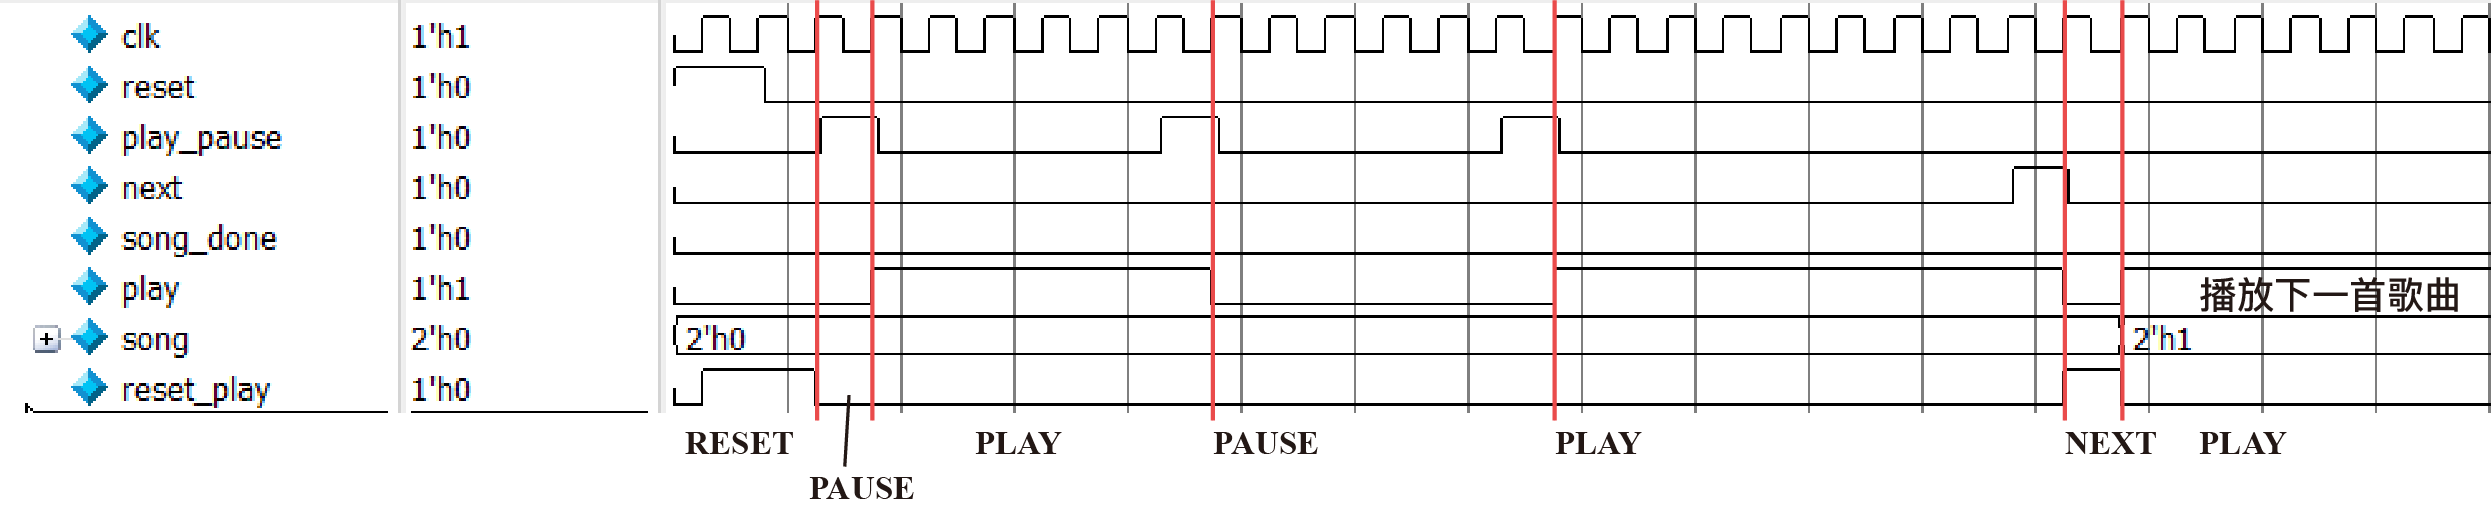
\includegraphics[width = 1\textwidth]{mcu-sim}
                    \caption{mcu仿真图}
                \end{figure}
            仿真分析:

            \begin{enumerate}
                \item 开始reset = 1,clk上沿到来时,电路处于RESET状态,输出play = 0,nextsong = 0,reset\_ play = 1。 
                \item 第一条红线时,reset = 0,play \_ pause = 0,电路进入PAUSE状态。
                \item 第二条红线时,reset = 0, play \_ pause = 1,相当于按下paly按钮,电路进入PLAY状态,play = 1。 
                \item 第三条红线时,reset = 0,play\_ pause = 1,电路进入PAUSE状态,输出play = 0。 
                \item 第四条红线时,reset = 0, play\_ pause = 0,next = 1,相当于按下next按钮,电路进入NEXT状态。
            \end{enumerate}

            \subsubsection{乐曲读取song \_ reader模块}
                \begin{figure}[H]
                    \centering
                    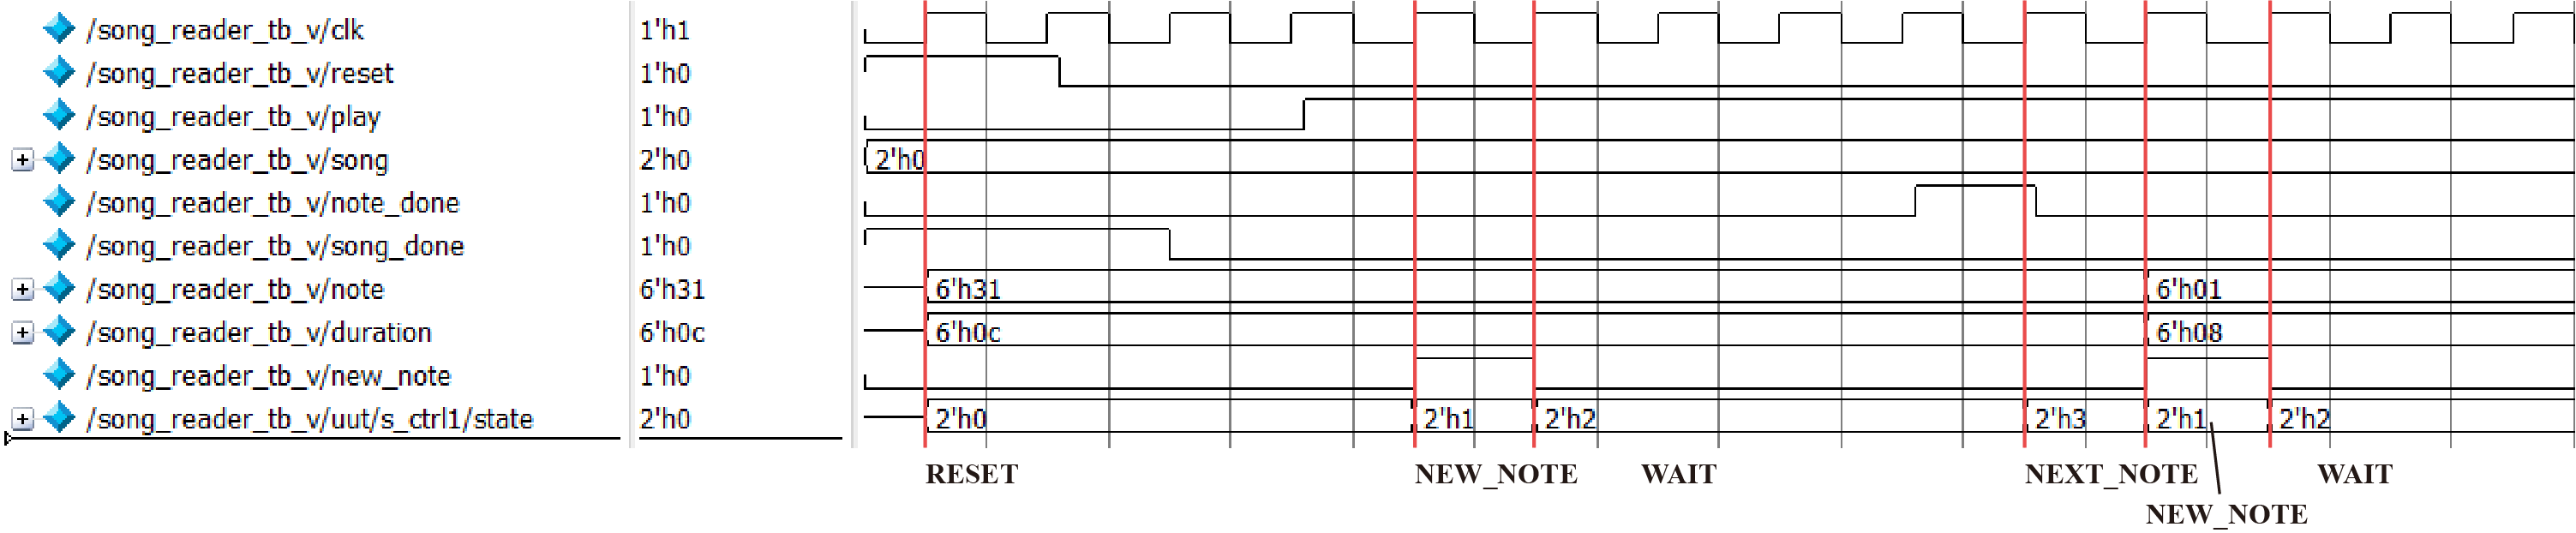
\includegraphics[width = 1\textwidth]{song-sim}
                    \caption{song \_ reader仿真图}
                \end{figure}

            仿真分析:

            \begin{enumerate}
                \item 第一条红线时,reset = 1, 电路进入RESET状态。
                \item 第二条红线时,reset = 0, play = 0,电路保持RESET状态。
                \item 第三条红线时,reset = 0, play = 1,电路接收到mcu发来的播放命令,进入NEW\_ NOTE状态,new \_ note = 1,要求note\_ player模块播放音符。 
                \item 第四条红线时,电路进入WAIT状态,等待播放停止或者音符播放完毕。
                \item 第五条红线时 ,note\_ done = 1,音符播放完毕,电路进入NEXT\_ NOTE状态,以延迟一个时钟周期输出信号,配合song\_ rom 的读取要求。
                \item 第六条红线时 ,电路进入NEW\_ NOTE状态,播放新的音符。
            \end{enumerate}
            \subsubsection{音符播放note \_ player模块}
                \begin{figure}[H]
                    \centering
                    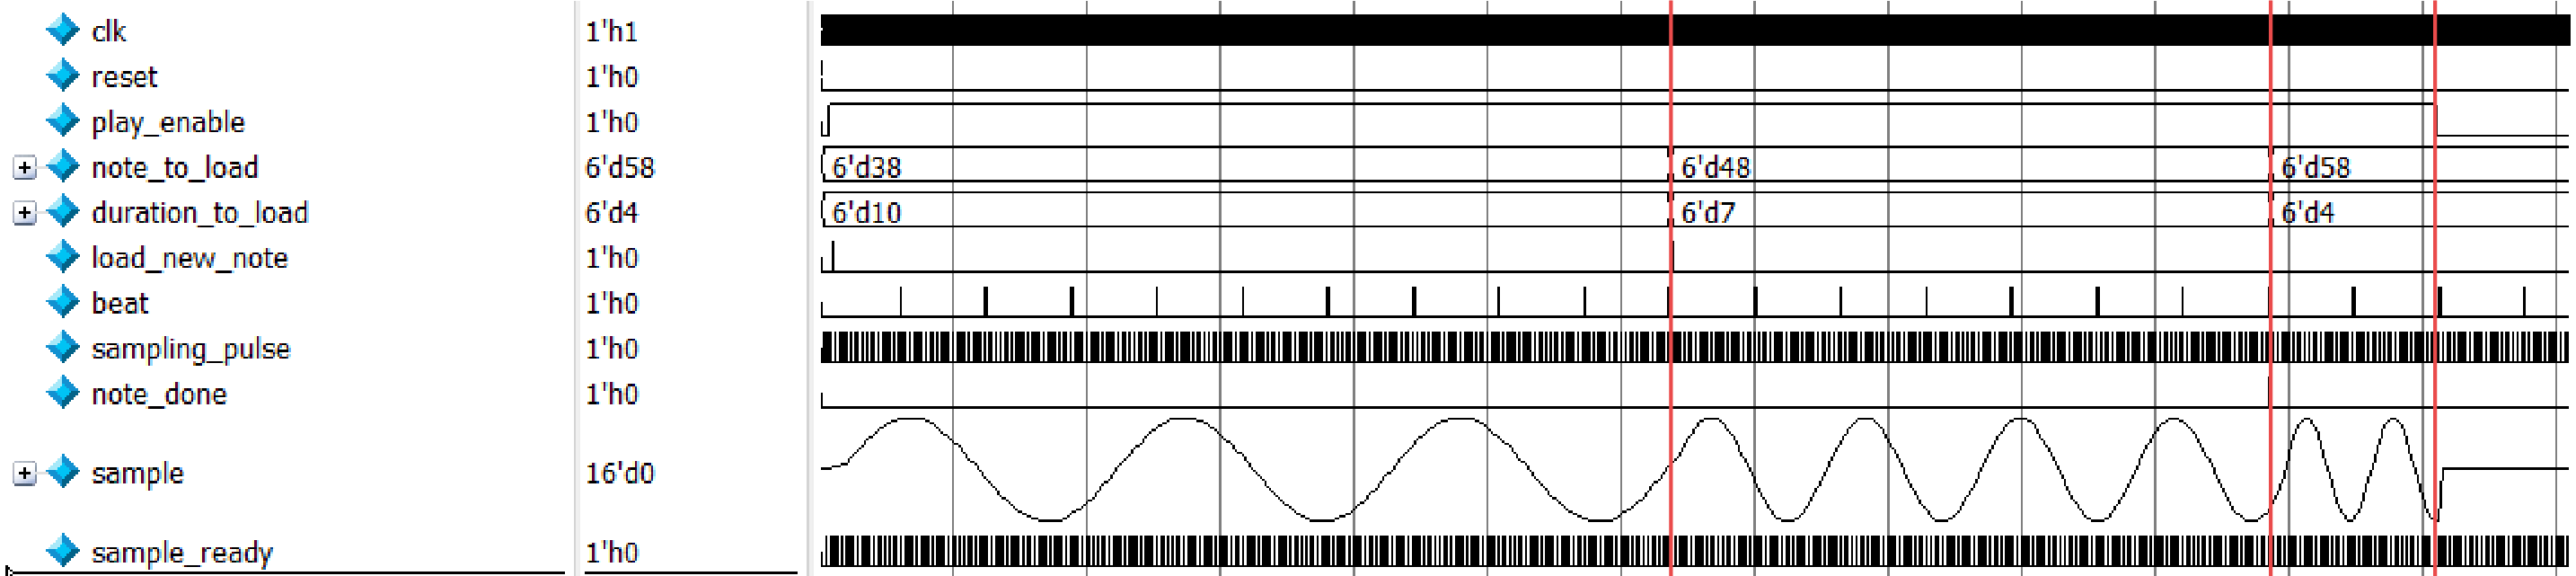
\includegraphics[width = 1\textwidth]{note-sim}
                    \caption{note \_ player仿真图}
                \end{figure}

            仿真分析:
            
            由仿真图可知,正弦波形的频率与note \_ to\_ load 的值呈正相关。同时只有当play \_ enabe = 1时才会输出波形。

            \subsubsection{次顶层music \_ player}
                \begin{figure}[H]
                    \centering
                    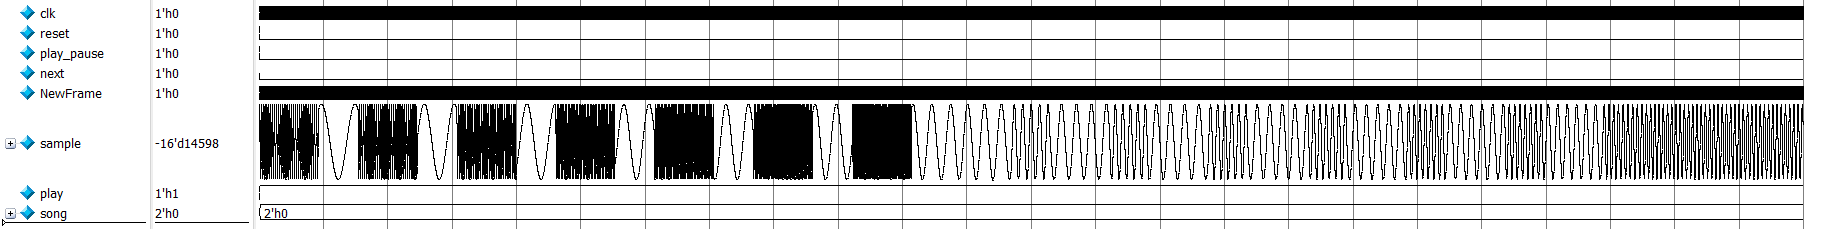
\includegraphics[width = 1\textwidth]{music}
                    \caption{次顶层music\_ player仿真图}
                \end{figure}
            根据仿真图,波形基本符合要求。

        \subsection{vivado实现}
            \begin{figure}[H]
                \centering
                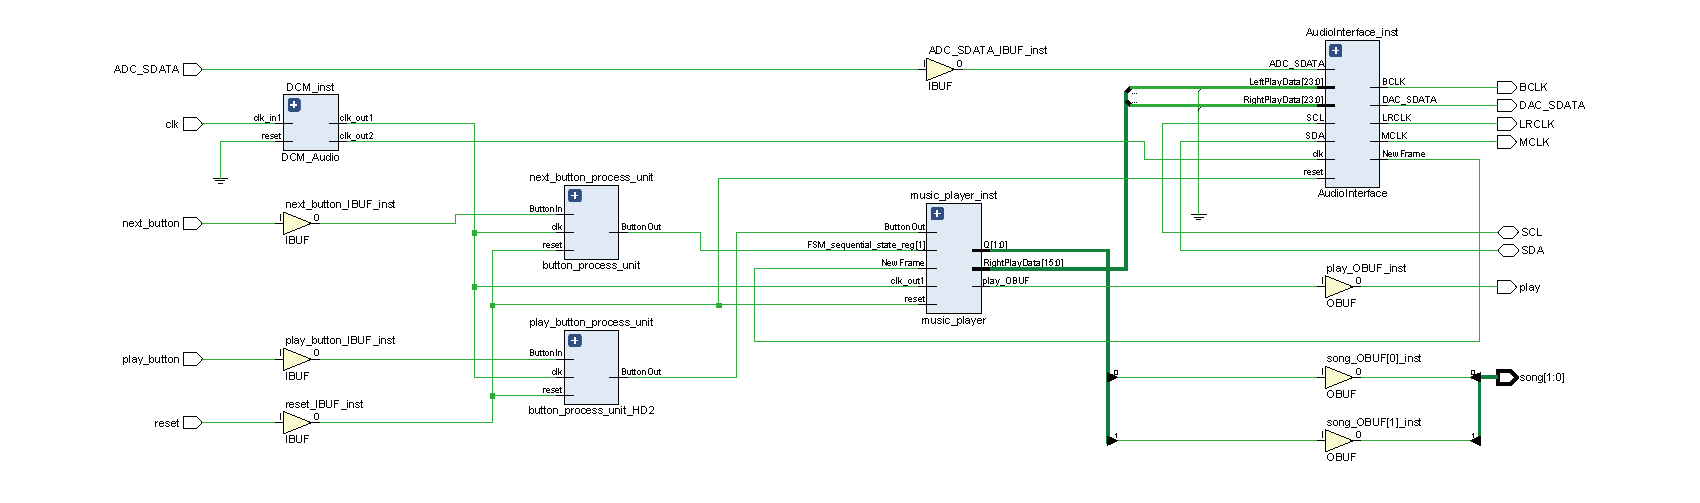
\includegraphics[width = 1\textwidth]{schematic}
                \caption{vivado实现}
            \end{figure}
        \subsection{实验中遇到的问题和解决方法}
            \begin{enumerate}
                \item 在最终上板测试阶段,发现播放歌曲的时候,当播放完毕时,无法自动停止。在老师的指导下,发现是我song \_ reader模块的结束判断代码出了问题。具体表现在我将判断条件duration = 0在代码中写成了$\sim$duration,但是由于duration并非1位数据,所以不能用简单的取反判断,应该用按位取反或duration == 0作为判断条件。在修改判断条件为duration ==0后,问题得到了解决。
            \end{enumerate}
    \section{思考题}
        \subsection{在实验中,为什么next\_button、play\_pause\_button两个按键需要消颤动及同步化处理,而reset按键不需要消颤动及同步化处理?}
        因为reset是置零信号,当reset=1时,系统置零,之后reset为0或为1系统内部该置零的信号都为0,reset的颤动对系统无影响。而next\_button和 play \_pause\_button 都会影响系统内部状态的转换,如果next输入不稳定,则不能达到播放下一首的目的,可能会跳到后面几首歌,也就是会使播放的下一首歌不确定;如果play\_pause 输入不确定,则系统会不断地在播放和暂停之间切换,这不仅会增加系统的损耗,而且会输出断断续续的音乐,达不到预期效果。
        \subsection{在主控制器(mcu)设计中,是否存在接收不到按键信息﹖若存在,概率多大?有没必要修改设
        计?}
        存在。在RESET到 PAUSE状态转换过程中和NEXT到 PLAY状态转换过程中没有判断 next和play\_pause,这期间按下按钮接收不到按键信息。概率很小,因为只有一个时钟周期,因此没有必要修改设计。
    
    \section{实验心得}
    本次实验一开始我其实是无从下手的。所以我就按照老师的建议,去做了前的涉及到的DDS子实验。在花了半天的时间后,我完成了DDS实验。然后我去看了老师提供的视频,学会了二段式描述中状态机。

    之后我便开始了最后的实验,一开始面对复杂的次顶层,我不知道从何开始,于是我便一个小模块一个小模块的设计。并且每个小模块的顶层文件和调用的子模块分开写,保证文件管理的清晰明确。

    在设计完一个一个的小模块之后,一开始觉得复杂的次顶层也慢慢变得清晰简单起来。最后也顺利完成了实验。
\end{document}